
% Annual Cognitive Science Conference
% Sample LaTeX Paper -- Proceedings Format
% 

% Original : Ashwin Ram (ashwin@cc.gatech.edu)       04/01/1994
% Modified : Johanna Moore (jmoore@cs.pitt.edu)      03/17/1995
% Modified : David Noelle (noelle@ucsd.edu)          03/15/1996
% Modified : Pat Langley (langley@cs.stanford.edu)   01/26/1997
% Latex2e corrections by Ramin Charles Nakisa        01/28/1997 
% Modified : Tina Eliassi-Rad (eliassi@cs.wisc.edu)  01/31/1998
% Modified : Trisha Yannuzzi (trisha@ircs.upenn.edu) 12/28/1999 (in process)
% Modified : Mary Ellen Foster (M.E.Foster@ed.ac.uk) 12/11/2000
% Modified : Ken Forbus                              01/23/2004
% Modified : Eli M. Silk (esilk@pitt.edu)            05/24/2005
% Modified : Niels Taatgen (taatgen@cmu.edu)         10/24/2006
% Modified : David Noelle (dnoelle@ucmerced.edu)     11/19/2014
% Modified : Roger Levy (rplevy@mit.edu)     12/31/2018

%% Change "letterpaper" in the following line to "a4paper" if you must.

\documentclass[10pt,letterpaper]{article}

\usepackage{cogsci}
\usepackage{mathrsfs}  
\usepackage{graphicx}  
\usepackage{tipa}
\usepackage{booktabs}
\usepackage{tikz}
\cogscifinalcopy % Uncomment this line for the final submission 


\usepackage{pslatex}
\usepackage{apacite}
\usepackage{float} % Roger Levy added this and changed figure/table
                   % placement to [H] for conformity to Word template,
                   % though floating tables and figures to top is
                   % still generally recommended!

%\usepackage[none]{hyphenat} % Sometimes it can be useful to turn off
%hyphenation for purposes such as spell checking of the resulting
%PDF.  Uncomment this block to turn off hyphenation.
\usepackage{color}
\definecolor{Red}{RGB}{255,0,0}
\newcommand{\red}[1]{\textcolor{Red}{#1}}
\newcommand{\jd}[1]{\textcolor{Red}{[jd: #1]}}
\definecolor{Blue}{RGB}{0,100,255}
\newcommand{\blue}[1]{\textcolor{Blue}{#1}}
\newcommand{\lk}[1]{\textcolor{Blue}{[lk: #1]}}

\newcommand{\tableref}[1]{Table \ref{#1}}
\newcommand{\figref}[1]{Figure \ref{#1}}

%\setlength\titlebox{4.5cm}
% You can expand the titlebox if you need extra space
% to show all the authors. Please do not make the titlebox
% smaller than 4.5cm (the original size).
%%If you do, we reserve the right to require you to change it back in
%%the camera-ready version, which could interfere with the timely
%%appearance of your paper in the Proceedings.

\title{Probability and processing speed of scalar inferences is context-dependent}
 
% \author{{\large \textbf{Leyla Kursat}  {\normalfont and} \textbf{Judith Degen}}  \\
%  \{lkursat, jdegen\}@stanford.edu \\
%   Department of Linguistics, Stanford University \\
%   Stanford, CA 94305, USA}

\author{{\large \textbf{names}}  \\
 \{names\}@school\\
  Address}

\begin{document}

\maketitle

%\renewcommand{\citeA}{\textbf}
%\renewcommand{\cite}[1]{\textbf{(#1)}}

\begin{abstract}

 The past two decades have seen a wealth of studies addressing the question of whether or not scalar inferences -- whereby a listener takes a sentence like \textit{Alex ate some of the cookies} to mean that he did not eat all of them -- generally incur a processing cost, with conflicting results. This has spurred the development of studies seeking to understand the contextual conditions that facilitate scalar inferences. Here, we test a prediction made by \citeA{DegenTanenhaus2015}'s constraint-based account: that the probability of an interpretation and the speed with which it is processed is a function of the contextual support it receives. We manipulated the contextual support for the scalar inference in two truth-value judgment experiments  via the manipulation of a lexical feature (presence of partitive ``of the``) and a pragmatic feature (the implicit Question Under Discussion). Participants' responder type -- whether they generally produced pragmatic responses reflecting the inference or literal responses reflecting its absence -- was the main predictor of response times: pragmatic responses  were faster than literal responses when generated by a pragmatic responder, whereas the reverse was true for literal responders. This suggests that, rather than generally incurring a processing cost, inferences are easy to process by listeners who take the context to generally support the inference, and hard to process by listeners who take the context not to support the inference. We interpret this as evidence against literal-first or costly-implicature accounts and in support of constraint-based accounts of pragmatic processing.\jd{include additional notes on subtle conntext effects?}

\textbf{Keywords:} psycholinguistics; experimental pragmatics; scalar implicature; Question Under Discussion

\end{abstract}

\section{Introduction}

\jd{this is still the elm abstract -- need to flesh out each part in more detail}

\begin{itemize}
	\item \jd{there are conflicting results regarding the question of whether or not inferences are costly to compute}
	\item \jd{dt have suggested that this is because inferences aren't generally costly or not costly -- instead, inference robustness and processing speed is a function of the contextual support it receives}
	\item \jd{while the contextual conditions that facilitate inference from `some' to `not all' have been increasingly well studied in the past few years -- showingn effects of contextual features x, y, and z on si -- the extent to which processing speed is a function of contextual conditions is still very much up in the air}
	\item \jd{we test the constraint-based account by manipulating features of context that provide variable support for the inference and test whether contextual support predicts response times}
	\item \jd{high-level description of the paradigm and the two contextual features}
\end{itemize}

The past two decades have seen a wealth of studies addressing the question of whether or not scalar inferences -- whereby a listener takes a sentence like \textit{Alex ate some of the cookies} to mean that he did not eat all of them -- generally incur a processing cost, with conflicting results \cite{BottNoveck2004,HuangSnedeker2009,Grodner2010,Breheny2013,DegenTanenhaus2016}. This has spurred the development of studies seeking to understand the contextual conditions that facilitate scalar inferences \cite{Zondervan2010,Degen2015,Augurzky2019,MartyChemla2013,DegenGoodman2014}.

Here, we test a prediction made by \citeA{DegenTanenhaus2015}'s constraint-based account: that the probability of an interpretation and the speed with which it is processed is a function of the contextual support it receives. In contrast, if scalar inferences generally incur a processing cost, pragmatic responses reflecting that the scalar inference was drawn should be slower to process than literal responses regardless of context. To test the constraint-based versus the costly inference account, we manipulated two features of context between participants in a truth-value judgement task: one lexical (\textit{presence of partititve "of"}) and one pragmatic (\textit{implicit QUD, see (1) and (2)}). This allowed us to obtain estimates of inference rate and processing speed. We further considered a participant’s \textit{responder type  --} whether they have a preference to respond literally or pragmatically -- as a predictive feature for response times. While the partitive and the QUD have previously been shown to affect the probability of drawing a scalar inference \cite{Zondervan2010,Degen2015,DegenGoodman2014,DegenTanenhaus2015}, contextual and participant-specific effects on processing speed have remained under-explored.

% \lk{can be moved to experimental paradigm section}
% Implicit QUDs (manipulated via cover stories as in \citeA{Degen2013}):
% \begin{enumerate}
%   \item Did I get all of the gumballs? (\textit{all}-QUD, \textit{more supportive of scalar inference})
%   \item Did I get any of the gumballs? (\textit{any}-QUD, \textit{less supportive of scalar inference})
% \end{enumerate} 

\section{Experimental paradigm}

\begin{figure}
\fbox{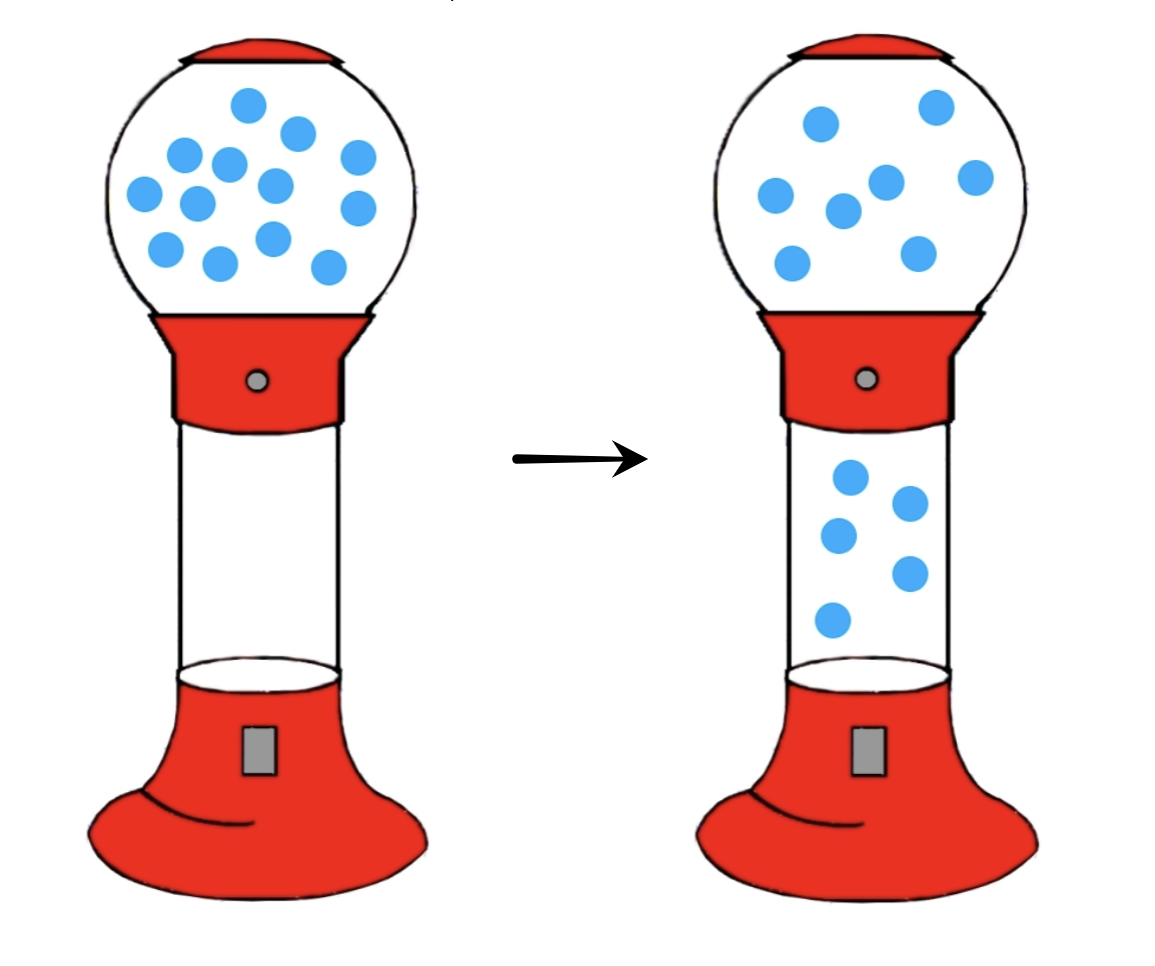
\includegraphics[width=\columnwidth]{./img/gumballs2.png}}
\caption{Example display from gumball paradigm. Left: initial display. Right: display with 5 gumballs dropped.  \label{fig:gumball-paradigm}}
\end{figure}

In both experiments, participants' interpretations were probed using the gumball paradigm introduced by \citeA{DegenTanenhaus2015}.  On each trial, participants saw a display of a gumball machine with 13 gumballs in the upper chamber and an empty lower chamber. After 4 seconds, some number of gumballs moved to the lower chamber and a voice reported how many gumballs were distributed (Fig.~\ref{fig:gumball-paradigm}). This pre-recorded statement was of the form "You got X gumballs", where X was a quantifier (\textit{some (of the)},  \textit{all of the}, \textit{none of the}, or a number between 1 and 13). The number of gumballs that dropped to the lower chamber and the quantifier  varied (see Table \ref{tab:stimuli}).

Participants were assigned to one of the two conditions (\textit{all}-QUD, \textit{any}-QUD) which differed in the cover story they were presented with at the beginning of the experiment (see Table \ref{tab:coverstories}). These cover stories were designed to establish the following implicit QUDs:
\begin{itemize}
\item \textbf{\textit{all}-QUD:} Is the machine empty? $\rightarrow$ Did I get all of the gumballs? (\textit{more supportive of scalar implicature})
\item \textbf{\textit{any}-QUD:} Is the machine jammed? $\rightarrow$ Did I get any of the gumballs? (\textit{less supportive of scalar implicature})
\end{itemize}

% \textbf{\textit{all}-QUD} Participants assigned to the \textit{all}-QUD condition read a cover story explaining that they are at a candy store helping the store worker test a row of special gumball machines. These gumball machines report how many gumballs they distribute but are sometimes incorrect in their report. Participants were also told that the store worker's boss has threatened to fire him if the gumaball machines are left empty and he cannot see the machines from the register and can only tell how full they are by their statements. Participants were asked to help the store worker by telling him if this statement is right or wrong by pressing the yes or no key. They were also told that they had 4 seconds to notify the store worker and they should make a decision as quickly as possible. 

% \textbf{\textit{any}-QUD} Participants in the \textit{any}-QUD condition read the same cover story except in their story, the gumball machines sometimes jam and don't deliver gumballs. The store worker's boss has threatened to fire him if the gumball machines stay jammed.

  \begin{table}
      \begin{tabular}{lccccccc}
      \midrule
      \multicolumn{8}{c}{\textbf{Set size}} \\
      \textbf{Quantifier} & 0 & 2 & 5 & 8 & 11 & 13 & \multicolumn{1}{l}{\textbf{Total}} \\
      \midrule
      \textit{some/some of} & 4 & 1 & 1 & 1 & 1 & 8 & 16 \\
      \textit{all of} & 2 & 1 & 2 & 1 & 2 & 8 & 16 \\
      \textit{none of} & 4 & 1 & 0 & 1 & 1 & 1 & 8 \\
      number & 3 & 7 & 7 & 7 & 5 & 3 & 32 \\
      \bottomrule
      \textbf{Total} & 13 & 10 & 10 & 10 & 9 & 20 & 72
      \end{tabular}
    \caption{Distribution of experimental trials over quantifiers and set sizes.\label{tab:stimuli}}
  \end{table}

  \begin{table*}[]
    \begin{tabular}{cclll}
      \cline{1-2}
      \toprule
      \textbf{all-QUD} & \textbf{any-QUD} &  &  &  \\
      \midrule
      \multicolumn{2}{c}{\begin{tabular}[c]{@{}c@{}}You are at a candy store and are testing a row of gumball machines. These are special \\ gumball machines that say how many gumballs you got. However, this report is \\ sometimes faulty.\end{tabular}} &  &  &  \\
      \midrule
      \begin{tabular}[c]{@{}c@{}}The store worker tells you that his boss has threatened \\ to fire him if the gumball machines are left empty, and he \\ really needs this job. He cannot see the machines from \\ the register, but he can normally tell how full they \\ are by the machines' statements.\end{tabular} & \begin{tabular}[c]{@{}c@{}}The store worker tells you that machines sometimes \\ jam and don't deliver any gumballs. His boss has \\ threatened to fire him if the gumball machines stay \\ jammed, and he really needs this job. He cannot see \\ the machines from the register, but he can normally \\ tell if they are working by the machines' statements.\end{tabular} &  &  &  \\
      \midrule
      \multicolumn{2}{c}{He asks you to tell him if the statement is right or wrong, so that he will know if a machine is empty and needs to be refilled.} &  &  &  \\
      \multicolumn{2}{c}{After you hear the statement, you have 4 seconds to notify the store worker, so please make a decision as quickly as possible.} &  &  & \\
      \bottomrule
      \end{tabular}
      \caption{Cover stories for each QUD condition.\label{tab:coverstories}}

  \end{table*}

\section{Experiment 1: Partitive statement}

In experiment 1 we tested whether the QUD, as a contextual feature of an utterance, could modulate the probability of a scalar implicature and the speed with which it is processed. The main prediction was that in the \textit{all}-QUD condition, the implicit QUD "Did I get all of the gumballs", would be more relevant to the "You got all of the gumballs" interpretation. Thus, there would be more pragmatic "disagree" responses in the critical trials when participants hear "You got some of the gumballs" and get all 13 gumballs. We also predicted that the relevance of the QUD would increase the speed of pragmatic responses and slow down the literal responses.

Procedure, materials, analyses and exclusions were pre-registered on OSF and will be available upon publication along with data and experiment scripts.

\subsection{Methods}

\paragraph{Participants}
We recruited 800 participants on Amazon Mechanical Turk. Participants were required to have a US-based IP address and a minimal approval rating of 95\%. They were paid \$2.30 (approximately \$14/hr).

\paragraph{Materials and procedure}
After reading the cover story of their QUD condition, participants went through a scripted demonstration that showed the consequences of store worker's responses to various scenarios. To ensure that they paid attention to the cover story, they were asked a multiple-choice question about the condition under which the store worker will be fired. When participants answered this question incorrectly, they were presented with the cover story again and had to repeat the demonstration. Halfway through the experiment, participants were asked to answer the multiple-choice question again. This was done to prevent the decay of the implicit QUD over time.

There were 4 practice trials with \textit{all} and \textit{none}. On half of these trials, the statements were correct, and on the other half they were incorrect. After the practice trials, there were 72 experimental trials (see Table \ref{tab:stimuli}). On 32 of the trials, the expected answer was yes, and on 32 of the trials, the expected answer was no. The remaining 8 trials were occurances of the critical trial and the main focus of this experiment. On these trials, all 13 gumballs dropped to the lower chamber and participants heard the partitive statement "You got \textit{some of} the gumballs". When participants press YES to agree with this statement, they interpret it semantically as "You got some, and possibly all, of the gumballs" and when they press NO to disagree, they interpret it pramatically as "You got some, but not all, of the gumballs". 

\noindent \textbf{Exclusions} We excluded participants who were self-reported non-native English speakers (n=26), participants who got the second cover story comprehension questions wrong more than twice (n=21) and participants with accuracy lower than 85\% on non-critical trials (n=185). Only responses to critical trials are reported below. These exclusions had no effect on the results discussed below. \lk{check again} 

\jd{i inserted the following; can also be excluded}
\noindent \textbf{Analysis and predictions} Only responses on critical trials are analyzed below. We conducted two types of analyses to address the two questions of interest:
\begin{enumerate}
\item Does the QUD modulate the probability of drawing a scalar inference?
\item Does the contextual support that an interpretation (either pragmatic or literal) receives
\end{enumerate} 
 To this end, we conducted a mixed effect logistic regression predicting the log odds of pragmatic ``no'' over literal ``yes'' responses. 
 
\subsection{Results and discussion}

\noindent \textbf{Judgments}

Proportion of pragmatic responses on critical trials are shown in Figure~\ref{fig:judgments}. 78\% of responses given by the participants in the \textit{all}-QUD condition were pragmatic compared to 71\% pragmatic responses given by participants in the \textit{any}-QUD condition. We ran a mixed effects logistic regression predicting response type with the maximal random effects structure justified by the design --  random by-participant intercepts -- from a fixed effect of QUD.  We observed a main effect of QUD such that there were more pragmatic responses in the \textit{all}-QUD condition compared to the \textit{any}-QUD condition ($\beta$=1.31, SE=0.52, p$<$.05).

\noindent \textbf{Analysis of Variability in Judgments} 

\figref{fig:proportion} shows the distribution of participants over number of pragmatic responses given on critical trials. Participants who either gave 0 or 8 pragmatic responses were completely consistent in their responses (62\%, of which 20\% completely literal and 80\% completely pragmatic). \figref{fig:proportion} mirrors \figref{fig:proportion} \lk{can make the plots seperately} and shows that the distribution of pragmatic responses in the \emph{all}-QUD condition is shifted towards the more pragmatic end of the continuum compared to the \emph{any}-QUD condition. Thus, while some participants were entirely consistent, there was also substantial inter-participant variability in consistency. For the purpose of the subsequent response time analyses, and following previous researchers \cite{BottNoveck2004,Degen2015}, we divided participants into two groups:  participants with more than 4 pragmatic responses were categorized as \emph{pragmatic} responders (74\%) and participants with fewer than 4 pragmatic responses were categorized as \emph{literal} responders (22\%). 15 participants (3\%) gave an equal number of pragmatic and literal responses and were excluded from the response time analysis. \jd{perhaps include a note saying what happens if the inconsistent people are included in a reasonable way?}

\begin{figure}
\centering
  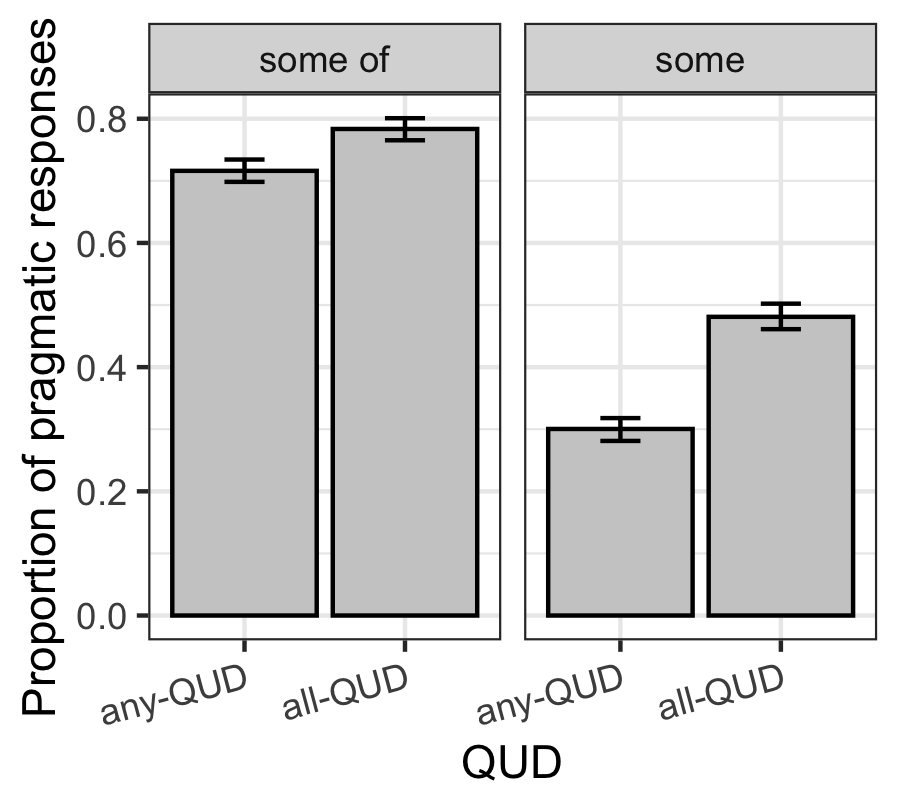
\includegraphics[width=.8\columnwidth]{plots/judgements.png}
  \caption{Proportion of pragmatic responses on partitive "some of" (left) and non-partitive "some" (right) critical trials. Error bars indicate bootstrapped 95\% confidence intervals. \label{fig:judgments}}
  \end{figure}
  
\noindent \textbf{Response Times} 

We predicted that the speed with which a scalar implicature is processed would increase with more contextual support. To test this hypothesis, we ran a mixed effects linear regression model with random by-participant intercepts predicting log-transformed response time from fixed effects of QUD, response type and their interaction. We found an interaction between QUD and response ($\beta$=-1.12, SE=2.51, t=-4.45, p$<$.0001) such that pragmatic responses were faster under the \textit{all}-QUD than under the \textit{any}-QUD. This shows that the relevance of an implicature to a contextual QUD modulates the speed of implicature processing. 

When we added responder type as predictor to this model, the largest observed effect was the interaction between responder type and response ($\beta$=-2.72, SE=3.34, t=-8.14, p$<$.0001), such that pragmatic responses were faster than literal responses for \emph{pragmatic}  responders and literal responses were faster than pragmatic responses for \emph{literal} responders (see Figure~\ref{fig:responsetimes}).

\begin{figure}
  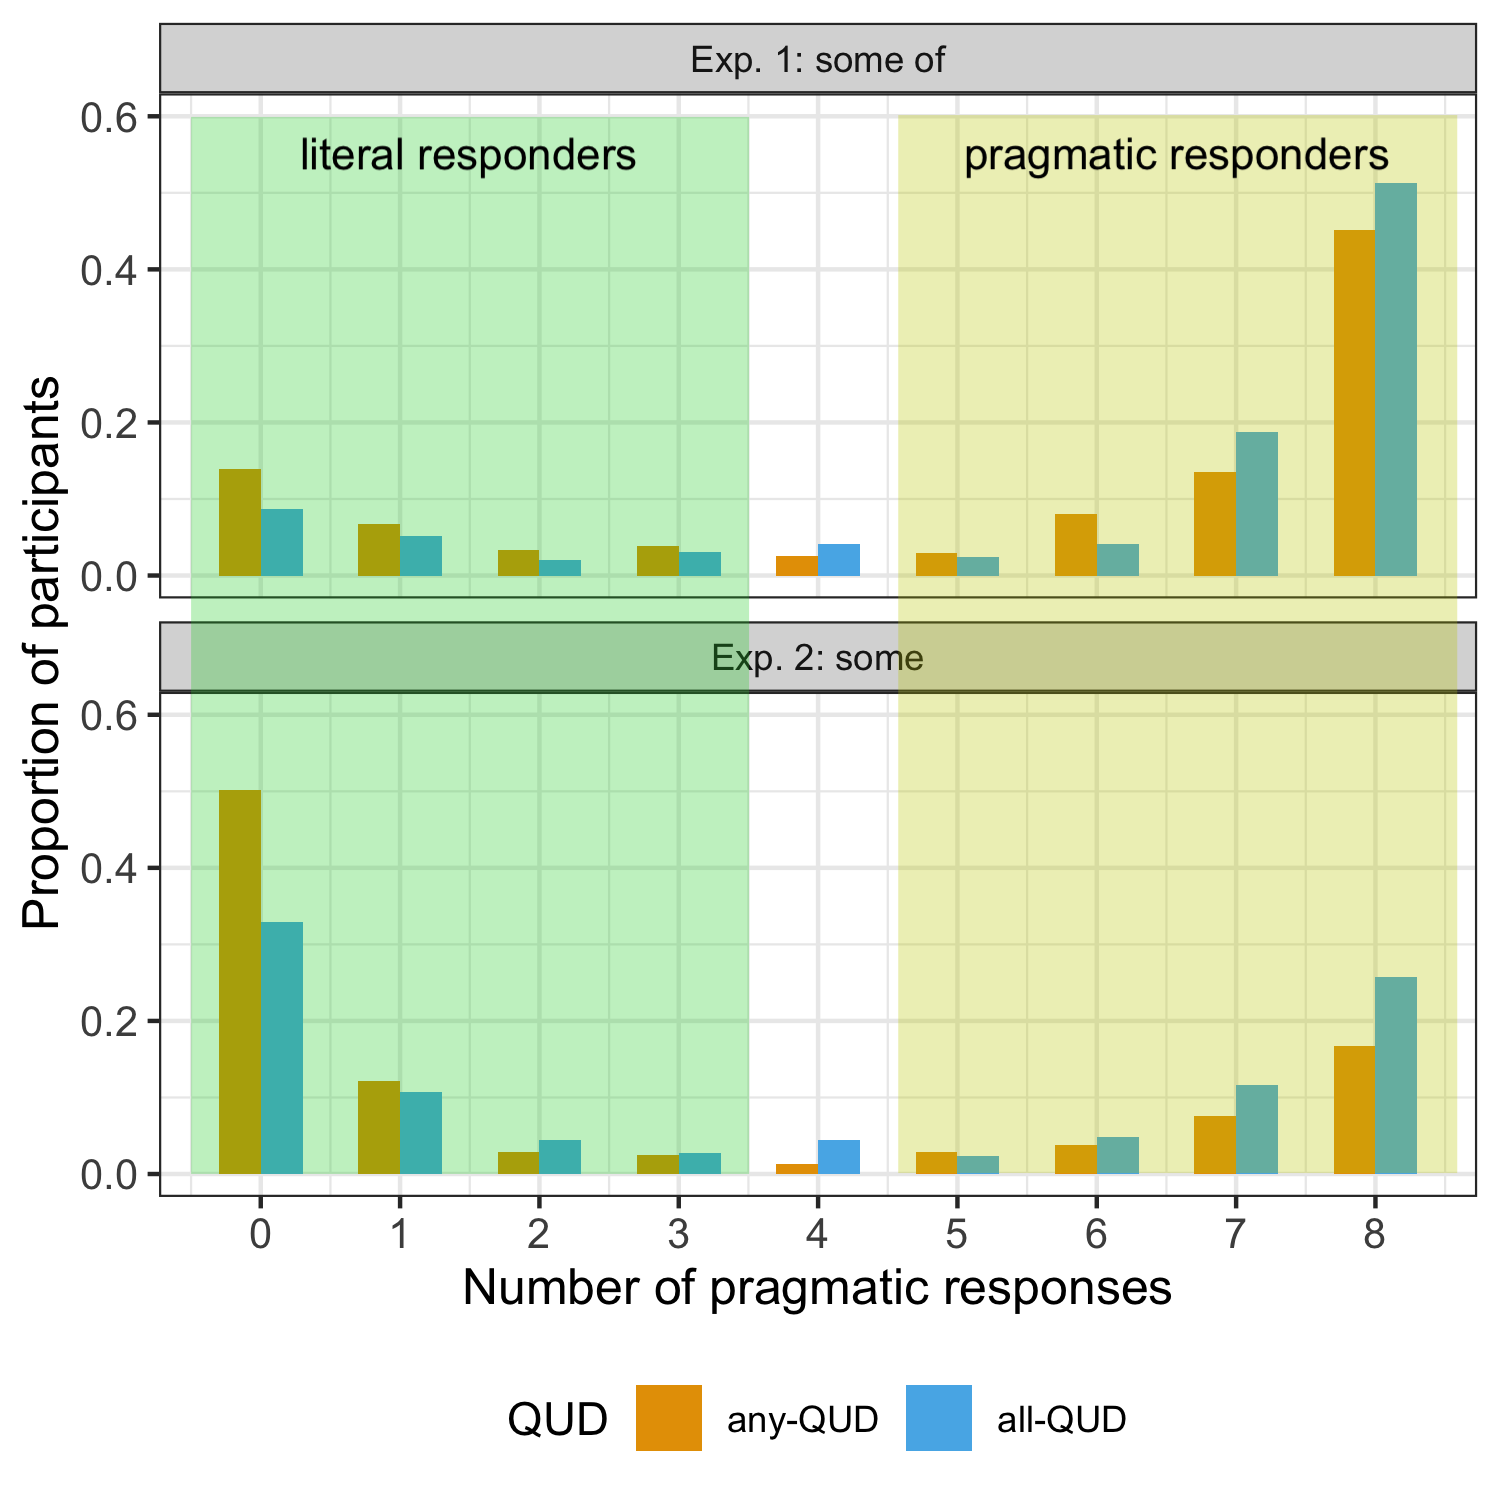
\includegraphics[width=\linewidth]{plots/proportion.png}
  \caption{Distribution of participants over number of pragmatic responses given on critical trials. Participants with $< 4$ pragmatic responses were categorized as literal responders (green), participants with $> 4$ responses as pragmatic responders (yellow). }
  \label{fig:proportion}
\end{figure}

\section{Experiment 2: Non-partitive statement}

In Experiment 2 we tested whether the absence of the partitive, previously shown to decrease the contextual support for the inference, would decrease the scalar inference rate. We also investigated whether the QUD and responder type effects observed in Experiment 1 would replicate without the contextual support of the lexical cue.

\subsection{Methods}

\noindent \textbf{Participants} We recruited 800 participants on Amazon Mechanical Turk. Participants had to have a US-based IP address and a minimal approval rating of 95\%, and they were paid \$2.3 (approximately \$14/hr).

\noindent \textbf{Materials and procedure} The materials and procedures were the same as in Experiment 1 except on critical trials, when all 13 gumballs dropped to the lower chamber, participants heard the non-partitive statement "You got \textit{some} gumballs".

\noindent \textbf{Exclusions} As in Experiment 1, we excluded non-native English speakers (n=21), participants who got the second comprehension question wrong more than twice (n=15), and participants that had accuracy lower than 85\% on non-critical trials (n=189).

\noindent \textbf{Analysis and predictions}
\jd{XXX}

\subsection{Results and discussion}

\begin{figure}
\centering
  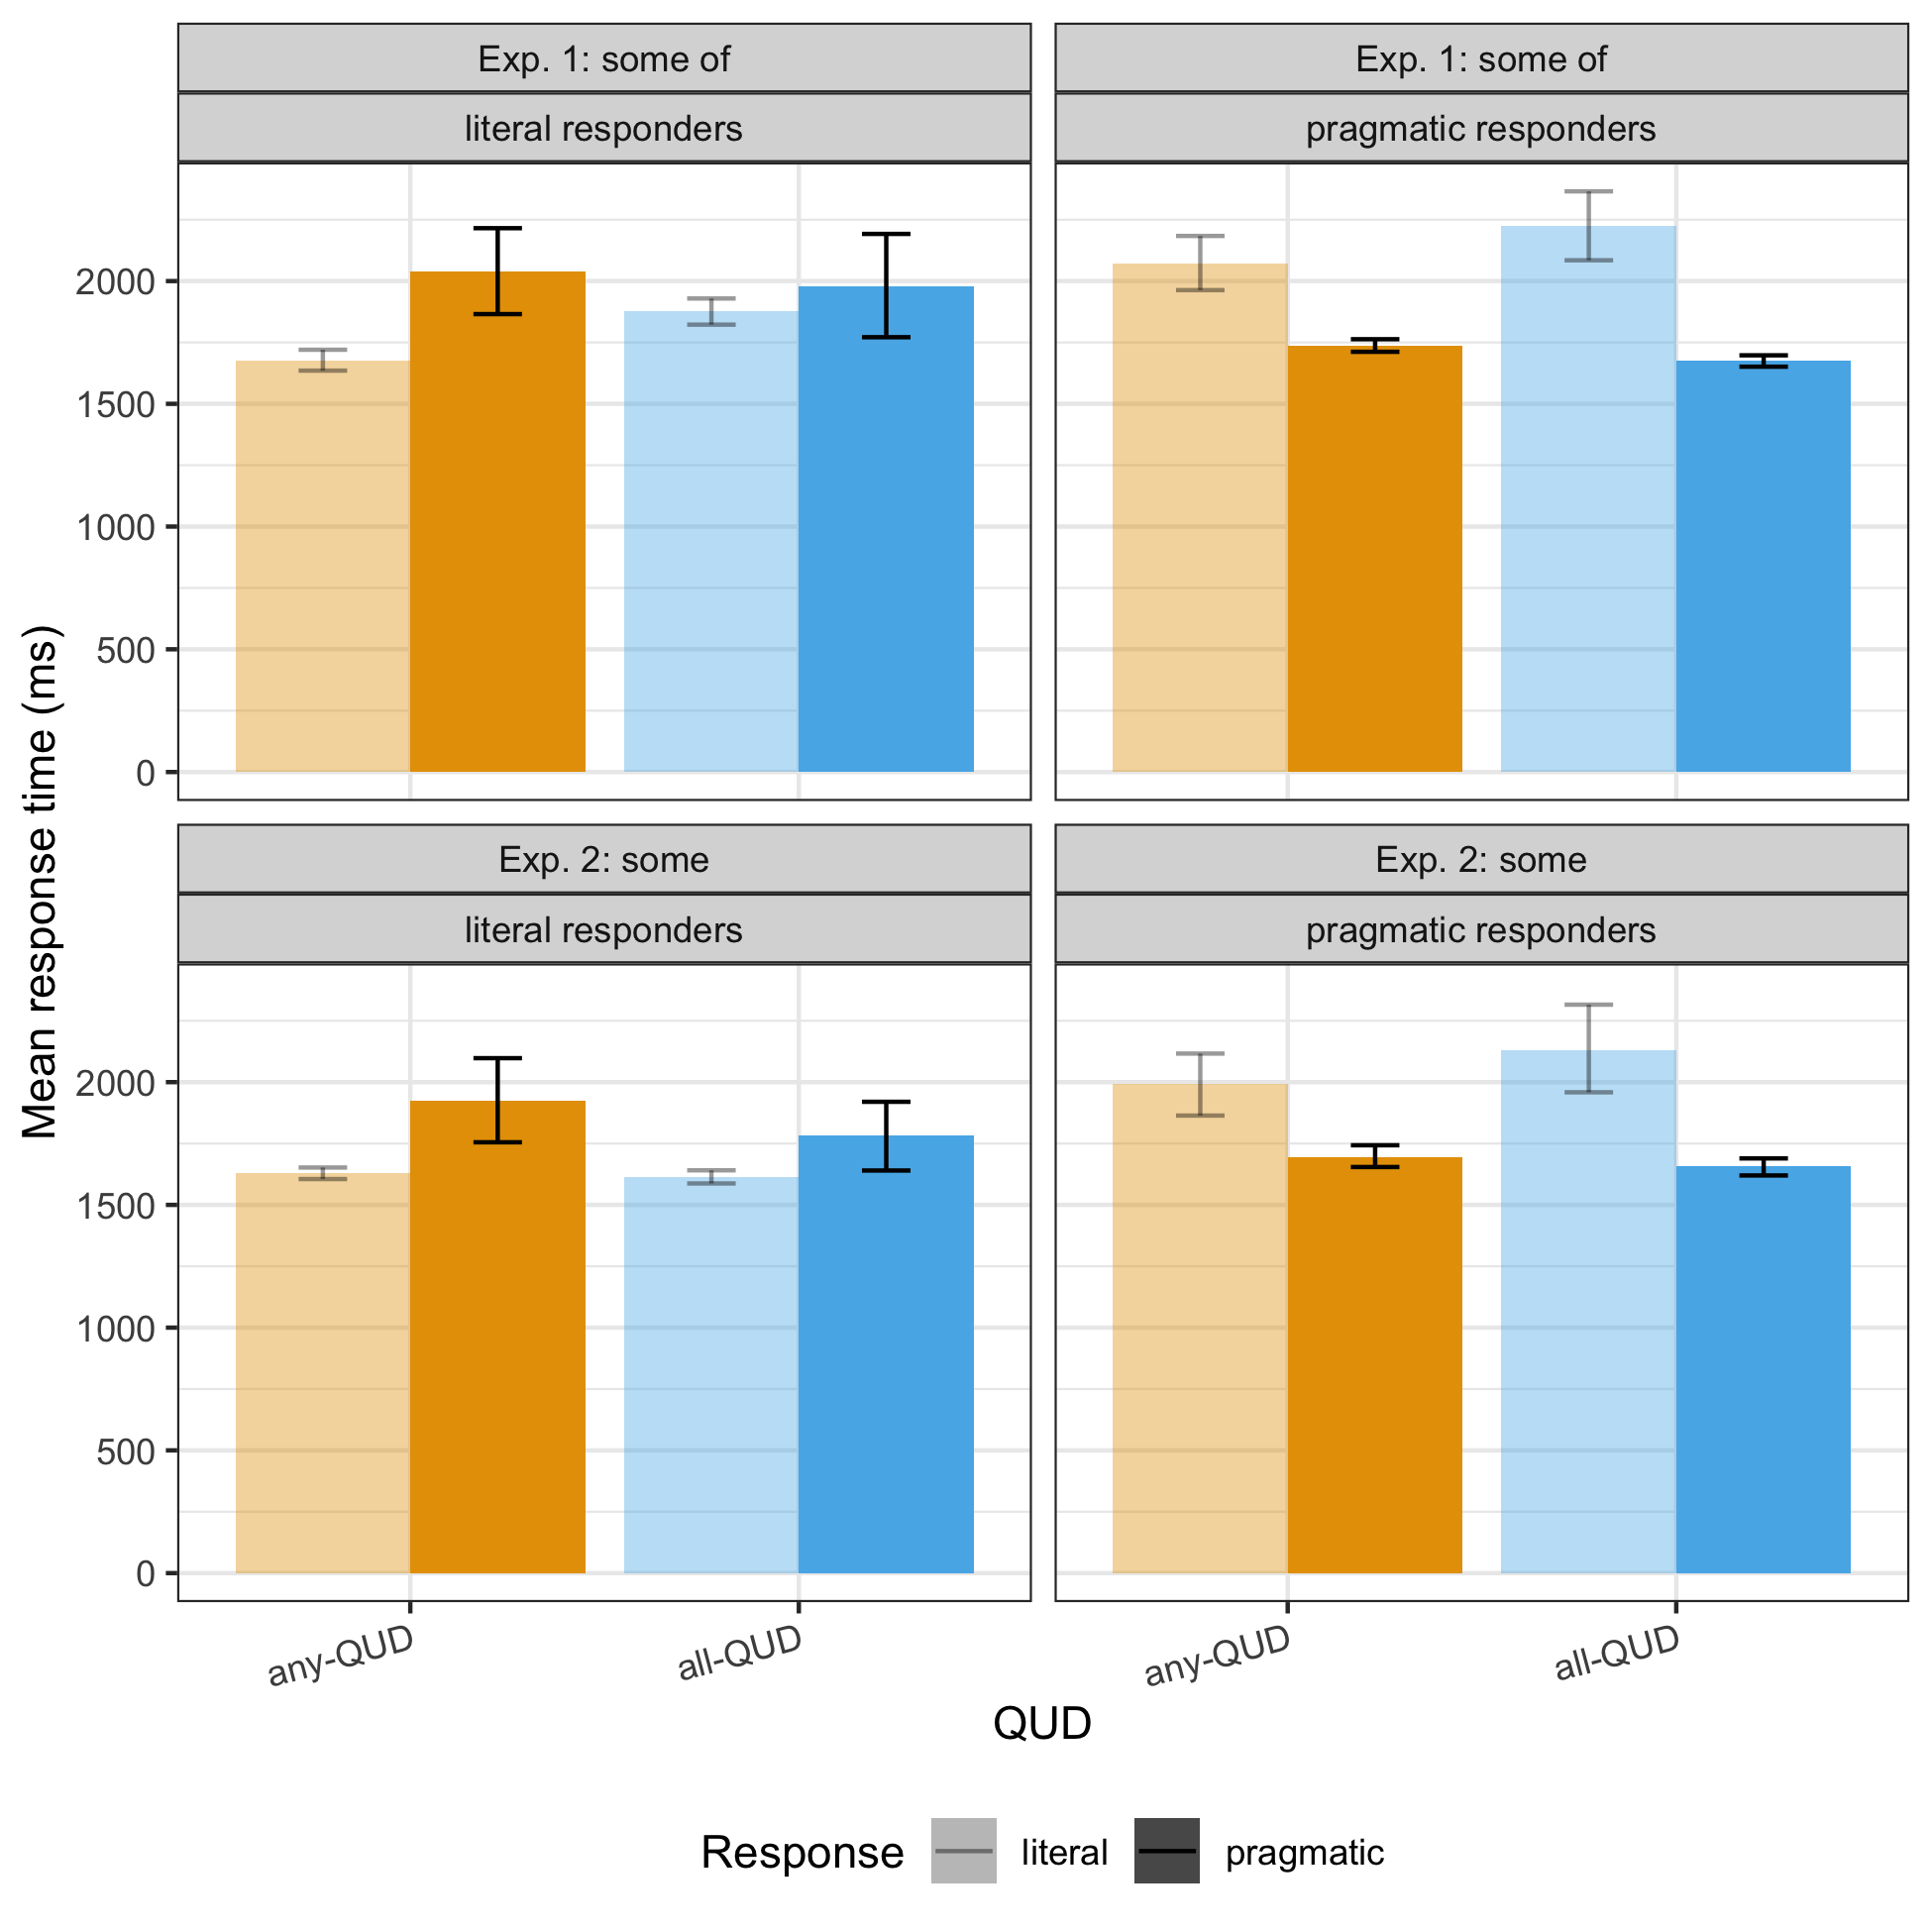
\includegraphics[width=\columnwidth]{plots/responsetimes}
  \caption{Mean response times for literal (light) and pragmatic (dark) responses generated by literal (left column) and pragmatic (right column) responders on partitive "some of" (top panels) and non-partitive "some" (bottom panels) critical trials. }
  \label{fig:responsetimes}
\end{figure}

\noindent \textbf{Judgments}

We found that overall, participants in Experiment 2 who heard the non-partitive statement were less likely to respond pragmatically compared to participants in Experiment 1 who heard its partitive counterpart ($\beta$=7.16, SE=0.69, p$<$.0001)(see Fig~\ref{fig:judgments}), replicating previous studies \cite{DegenTanenhaus2015,Degen2015}.

We also found an interaction of the lexical cue and QUD ($\beta$=-3.06, SE=0.90, p$<$.0001) but it was mainly because of the QUD effect being bigger for the non-partitive condition due to a ceiling effect. \lk{fix}

We replicated the QUD effect found in Experiment 1. Participants in the \textit{all}-QUD condition gave more pragmatic "disagree" responses than participants in the \textit{any}-QUD ($\beta$=4.69, SE=0.80, p$<$.0001). \lk{maybe say why we pool data} When we pooled the data from Experiment 1 and 2, QUD remained to be a predictor of response type ($\beta$=2.85, SE=0.44, p$<$.0001).

\noindent \textbf{Analysis of Variability in Judgments}

44\% of participants were completly consistent in their pragmatic responses compared to 20\% of participants that gave 0 pragmatic responses. 15 participants (3\%) were excluded from the response time analysis because they gave equal number of pragmatic and literal responses.

As shown in Fig~\ref{fig:proportion}, in the \emph{any}-QUD condition, the distribution of pragmatic responses is shifted towards the more literal end of the continuum compared to the \emph{all}-QUD condition. Overall, we see a shift \lk{complete opposites}

\noindent \textbf{Response Times}

In order to compare the response times of participants from Experiment 1 and 2, we had to calculate each response time with respect to the length of the audio stimuli participants heard. For each experiment, we subtracted the length of the onset of the word "gumball" (Experiment 1: 868ms, Experiment 2: 736ms) from all response times. This ensured that response times \lk{XXX}. We were interested in whether the lack of the partitive would slow down pragmatic responses and speed up literal responses compared to its partitive counterpart. We analyzed the data using a mixed effects linear regression model with by-participant intercepts to predict log-transformed response times. The model included centered fixed effects of quantifier and response. We found a significant interaction between quantifier and response such that ($\beta$=-0.10, SE=0.04, t=2.48 p$<$.05) \lk{explain}

\lk{
We weren't able to replicate the QUD effect on the speed of scalar implicatures when the non-partitive form was used.}

\lk{which one do we want to focus on?}
Finally, we ran a full model on the pooled data with QUD, quantifier, response and responder type as centered predictors. We found a main effect of quantifier ($\beta$=5.24, SE=1.52, t=3.45, p$<$.001), response ($\beta$=-8.69, SE=1.15, t=-7.58, p$<$.001), an interaction between qud and response ($\beta$=-1.06, SE=2.29, t=-4.62, p$<$.001), and an interaction between response and responder type ($\beta$=-2.69, SE=2.30 t=-11.68, p$<$.001)

% We also ran a full model on the pooled data and predicted log-transformed response times from centered fixed effects of QUD, quantifier, response and responder type. The model included by-participant intercepts. We found a main effect of partitive ($\beta$=5.24, SE=1.52, t=3.45, p$<$.001), an interaction between qud and response ($\beta$=-1.06, SE=2.29, t=-4.62, p$<$.001), and an interaction between response and responder type ($\beta$=-2.69, SE=2.30 t=-11.68, p$<$.001).


\section{General discussion and conclusion}

Contextual factors affect listeners' overall contextual response strategy which in turn impacts the speed with which they process the preferred interpretation. This is evidence against costly inferece accounts and in support of constraint-based accounts.

\begin{figure}
  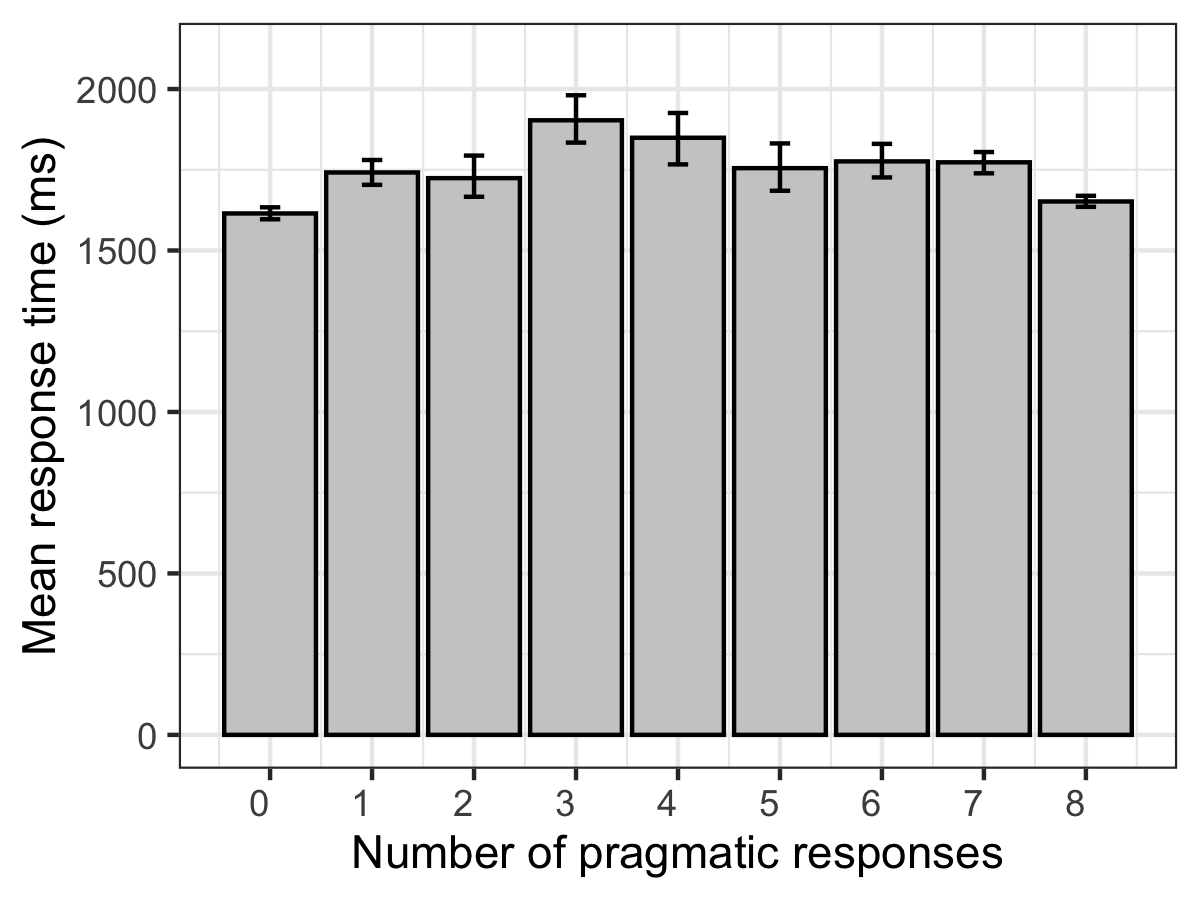
\includegraphics[width=\columnwidth]{plots/consistency.png}
  \caption{Mean response times for participants grouped based on the number of pragmatic responses they gave. \label{fig:consistency}}
\end{figure}

%\section{References Instructions}
%
%Follow the APA Publication Manual for citation format, both within the
%text and in the reference list, with the following exceptions: (a) do
%not cite the page numbers of any book, including chapters in edited
%volumes; (b) use the same format for unpublished references as for
%published ones. Alphabetize references by the surnames of the authors,
%with single author entries preceding multiple author entries. Order
%references by the same authors by the year of publication, with the
%earliest first.
%
%Use a first level section heading, ``{\bf References}'', as shown
%below. Use a hanging indent style, with the first line of the
%reference flush against the left margin and subsequent lines indented
%by 1/8~inch. Below are example references for a conference paper, book
%chapter, journal article, dissertation, book, technical report, and
%edited volume, respectively.


\bibliographystyle{apacite}

\setlength{\bibleftmargin}{.125in}
\setlength{\bibindent}{-\bibleftmargin}

\bibliography{cogsci}

\end{document}
